\documentclass{article}
\usepackage{graphicx}
\usepackage{amsmath,amssymb}
\usepackage{array}
\newcolumntype{$}{>{\global\let\currentrowstyle\relax}}
\newcolumntype{^}{>{\currentrowstyle}}
\newcommand{\rowstyle}[1]{\gdef\currentrowstyle{#1}%
  #1\ignorespaces
}
\usepackage[style=numeric-comp,backend=bibtex]{biblatex}
\bibliography{refs.bib} %Imports bibliography file

\title{Improving drug discovery by using molecular embeddings to augment high-content phenotypic screens}
\date{\today}
\author{Neil Thomas}

\begin{document}
\maketitle

\section{Project Description}

There is great demand for new compounds that could be used as drugs to treat disease. Drugs may be precisely targeted to subpopulations, or that can circumvent disease resistance. In addition, drugs may have many negative side effects: can similar therapeutic effects be found in different compounds with fewer side effects?

Testing massive libraries with tens of thousands of compounds for their biological effects is time consuming and expensive. To reduce this cost, recent research computationally explores the space of compounds using generative models (e.g. variational autoencoders). The parameter space of these generative models can be optimized over to maximize or specify the output of a predictor function (e.g. drug effect) \cite{Brookes2018} \cite{Gomez-Bombarelli2018}, see Figure \ref{chemvae} for a schematic of this process. This technique shows promise for designing new compounds with desired properties. However, meaningful predictors for complex biological activity are lacking, limiting the ability of generative models to generate molecules that effectively treat disease.

\begin{figure}[h]
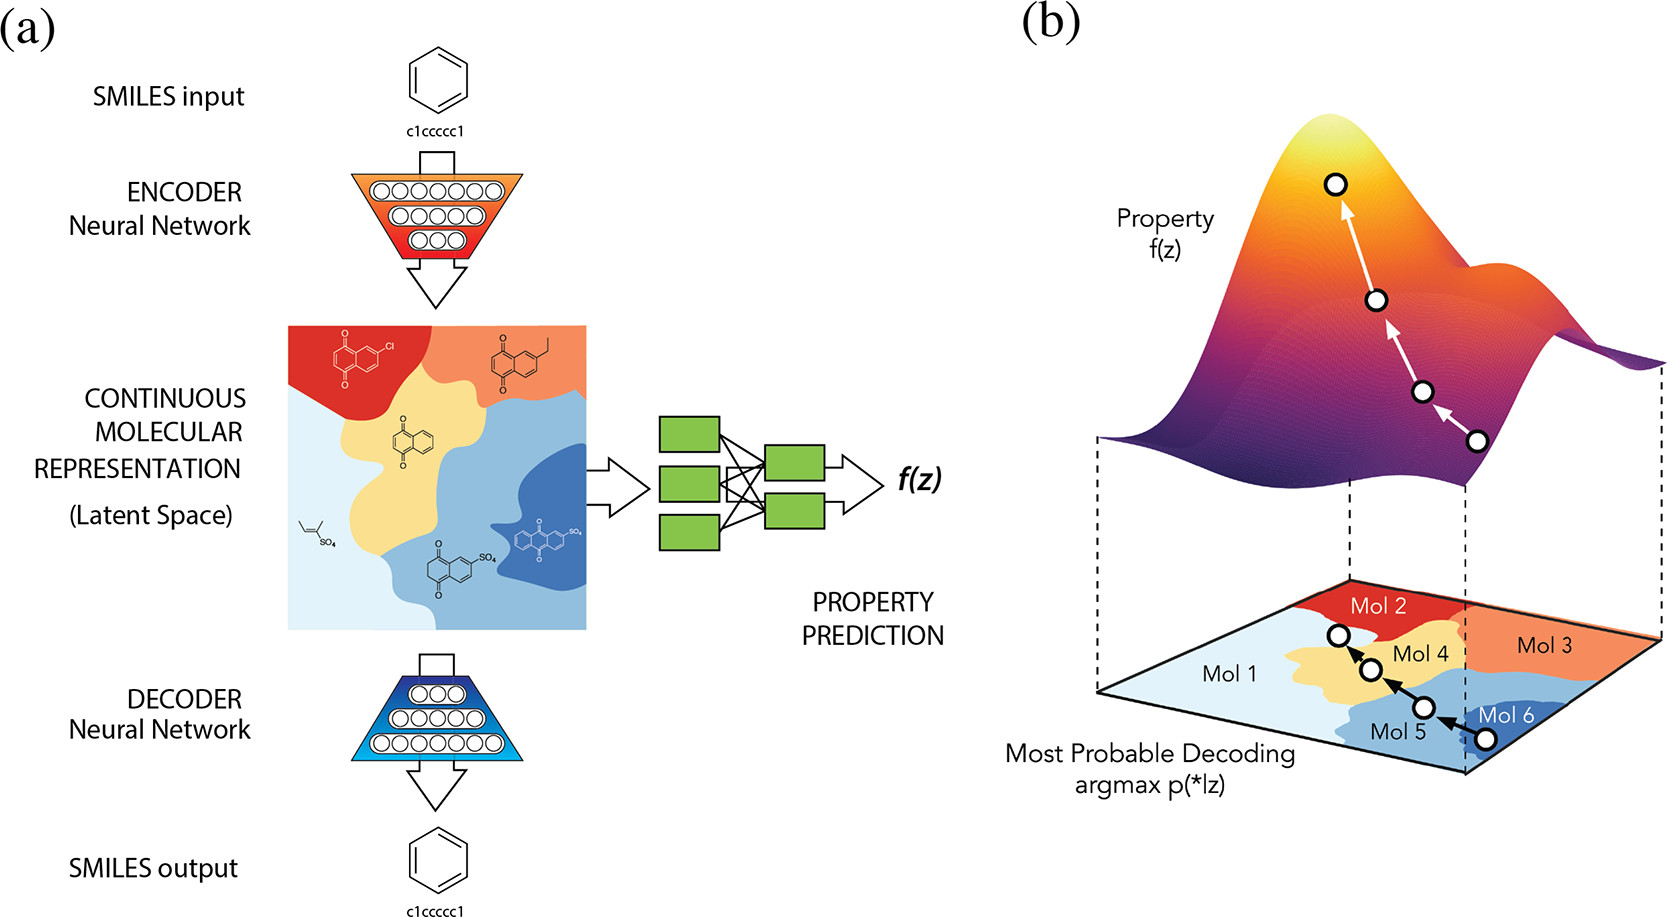
\includegraphics[width=\textwidth]{figs/chemvae.jpeg}
\caption{Training and optimizing over a chemical latent space in \cite{Gomez-Bombarelli2018}}
\label{chemvae}
\end{figure}

Recently, a low-cost, high-throughput drug screen that relies on imaging microscopy has been developed \cite{Kang2016}. This screen uses a single, optimally selected cell line with fluorescent labels on the cell membrane, nucleus, and a selected protein. Populations of cells are treated with each drug. Each sample is imaged pre-treatment and post-treatment (after 24h and 48h). The cumulative distribution functions (CDF) of 200 features encompassing cell morphology changes, protein localization, and other features are compared between pre and post-treatment using a Kolmogorov-Smirnov statistic. In this way, each drug can be summarized as a 200 dimensional vector associated with its cellular effect. Drugs which cluster far away from DMSO (an inactive solvent), and close to reference drugs of known effect, are shown to indeed affect similar pathways. For a schematic see Figure \ref{oracl_screen}.

\begin{figure}[h]
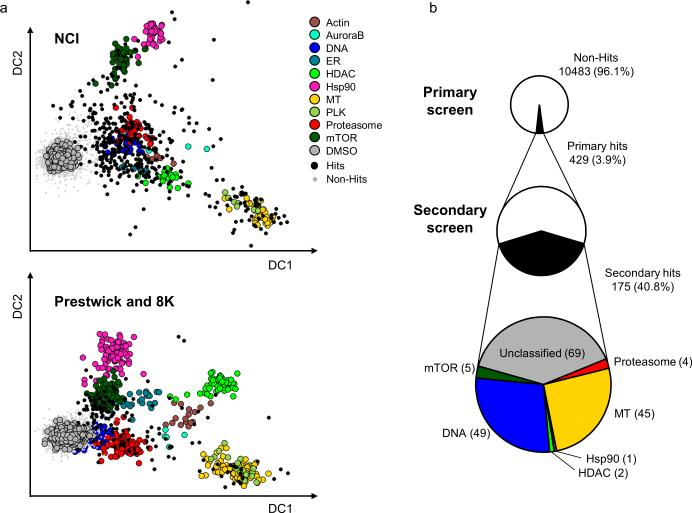
\includegraphics[width=\textwidth]{figs/oracl_screen}
\caption{Schematic overview of how clustering of drug effect vectors is used to screen for unknown drugs of similar function \cite{Kang2016}. Black dots are hits that cluster with reference compounds that affect known pathways (colored dots) and away from the inactive DMSO solvent (grey).}
\label{oracl_screen}
\end{figure}

These screens, however, do not utilize any prior information about similarity in molecular structure to help predict similarity in drug effect. It is all but axiom in biochemistry that similar structure connotes similar function. Can incorporating information about chemical structure help improve the precision (false positive rate) and/or recall (false negative rate) of these phenotypic screens?

One promising avenue for meaningfully summarizing structural similarity follows research from natural language processing, and the learning of word and document embeddings \cite{Goldberg2014}. By drawing the analogy of graphical substructures (rooted subgraphs) within a complete graph as ``words'' within a ``document'', similar word2vec intuition can be applied to learning $d$-dimensional continuous embeddings for arbitrary graph structures, deemed graph2vec \cite{Narayanan}. Graphs with similar substructures are similar graphs, and are close (in a Euclidean distance sense) in the embedding space. Since molecules can be represented as graphs, graph2vec embeddings can take advantage of large, unlabeled molecular datasets to learn rich embeddings that capture structural similarity between molecules. This also circumvents one of the problems with learning molecular embeddings via SMILES strings as in \cite{Gomez-Bombarelli2018}, as graph2vec does not need to learn the complex chemical syntax of SMILES. Word embeddings have already shown promise for being able to meaningfully capture biophysical characteristics of proteins and DNA sequences \cite{Hamid2018} \cite{Asgari2015}.

\section{Proposed Project Plan}

\subsection{Data collection}

The first step is to get access to the data from the phenotypic screening paper \cite{Kang2016}. In particular, we need to get access to the 200 dimensional feature vectors $v_f$ for each drug. We need to get the functional labels --- labels which specify the biological pathway of activity for each drug (e.g. mTOR inhibitor) --- for reference compounds used to design the screen, as well as additional known drug classes. We also need to get the validated hits from the original model (post-screening), so we can evaluate precision and recall for improvements to the model.

\subsection{Training the molecular embedding}

In order to do this, we need a large dataset of molecules. In \cite{Kang2016}, they have 10,916 compounds pooled from a number of different compound sets, including drug sets from the National Cancer Institute ($\sim$2000) and the University of Texas Southwestern 8K diversity subset ($\sim$8,000 compounds). graph2vec \cite{Narayanan} is validated on smaller datasets, including NCI datasets with $\sim$4000 compounds, so this dataset should be large enough to train a reasonable embedding. Each of these datasets will need to be transformed into a proper graphical format (using the graph API provided by the package networkx) to be used as input into graph2vec.

The graph2vec training algorithm is implemented at \url{https://github.com/MLDroid/graph2vec_tf}. This will need to be built, and run on the compound datasets. We plan to utilize GPU instances to speed up the training of the embedding.

Further experimentation will be necessary to determine the optimal dimension $d$ of the embedding, as well as whether embeddings are improved by including larger, non-cancer specific datasets, such as ZINC (250k compounds) or QM9 (100k compounds).

% more local embedding better?
\subsection{Validate the molecular embedding}

We will need to make sure that our molecular embedding is sensible. One way to do so is to evaluate the continuity of known oracle functions, such as water–octanol partition coefficient (logP) on the embedded space. In \cite{Gomez-Bombarelli2018} and \cite{Asgari2015} they do this qualitatively by examining a 2-dimensional projection (PCA or t-SNE, respectively) of the embedding space and examining the gradients in the desired features across compounds, see Figure \ref{chemvae_continuity}.

\begin{figure}[h]
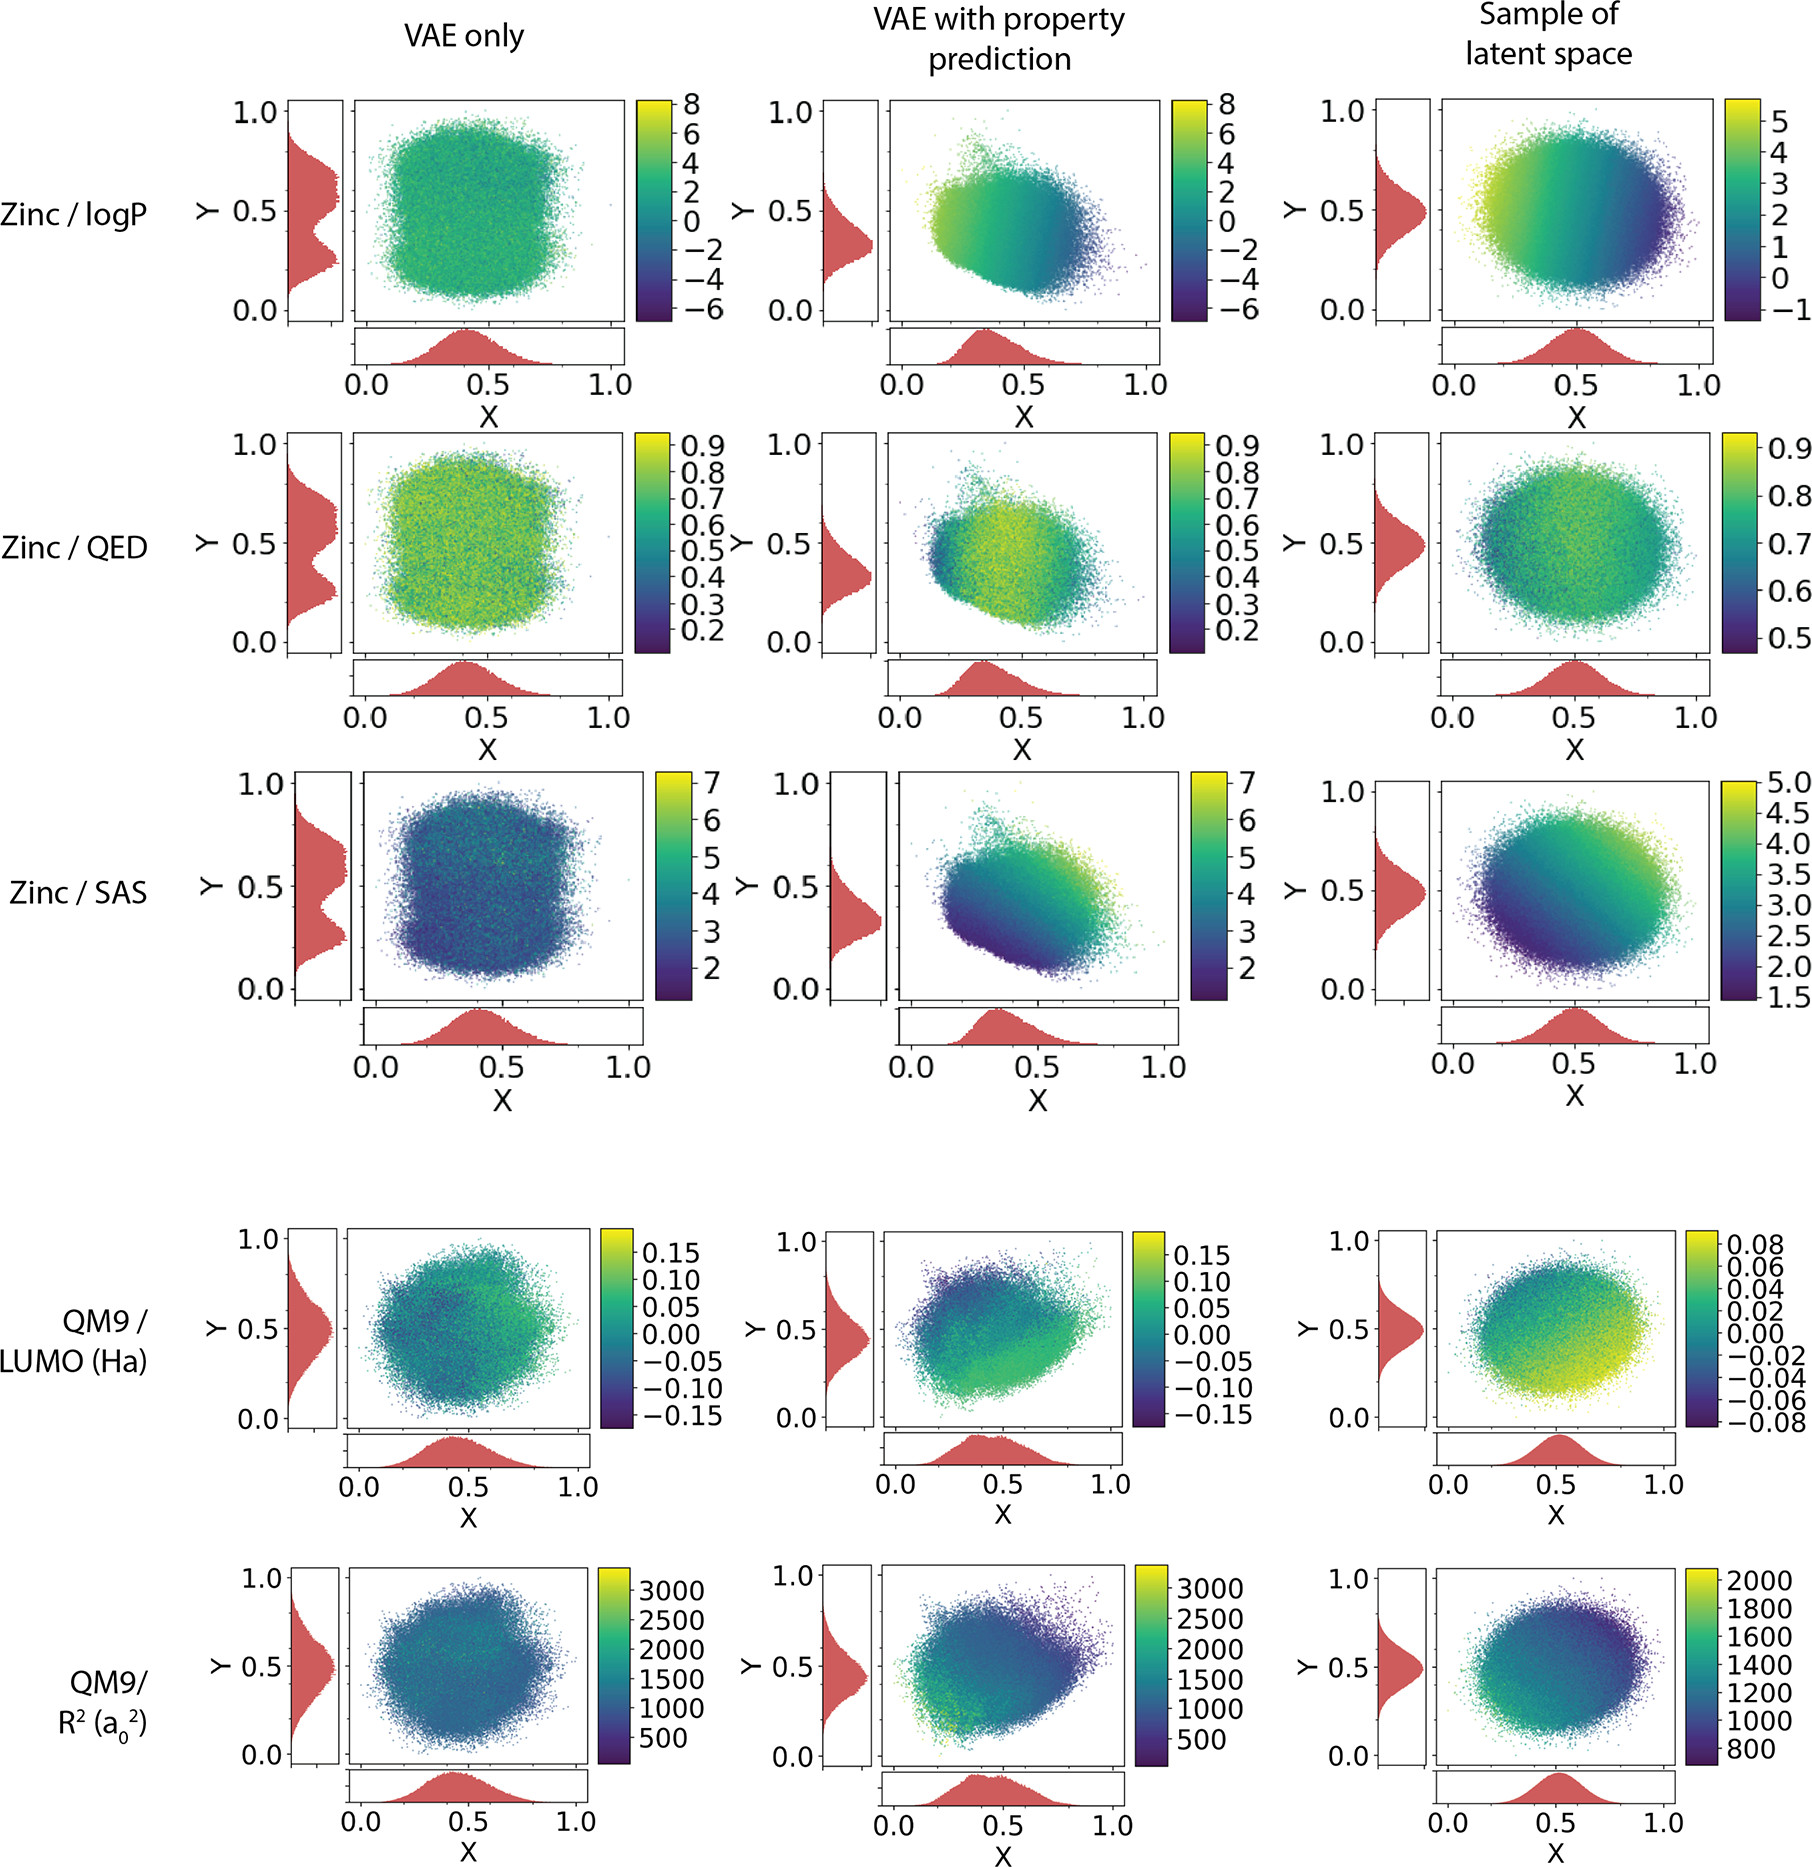
\includegraphics[width=\textwidth]{figs/chemvae_continuity.jpeg}
\caption{Evaluation of continuity of chemical latent space in \cite{Gomez-Bombarelli2018}}
\label{chemvae_continuity}
\end{figure}

\subsection{Incorporating molecular embeddings into phenotypic screening data}

The most immediate way to incorporate molecular embeddings would be to concatenate the $d$-dimensional graph embedding $v_g$ to the 200-dimensional feature vector $v_f$ and perform clustering on the resulting vectors $v = \left[v_f, v_g\right]$. Another potentially fruitful avenue to explore would be to use adaptive generalized Principal Components Analysis (gPCA) \cite{Fukuyama2017} to cluster compounds. Adaptive gPCA is a general method for incorporating prior information into clustering, which was originally applied to incorporate information about bacterial phylogenetic trees into clustering samples of 16S bacterial DNA sequences from human microbiota.

\subsection{Evaluate effectiveness of incorporating structure}

This is slightly tricky without access to further experiments to validate novel hits (e.g. check if a new labeled compound is indeed an mTOR inhibitor), but one criterion we can use to evaluate the new compound clusters is to see whether all of the validated hits make it through the new screen while reducing the number of invalidated hits. In addition, we would want to make sure that, in particular, drugs with differing structure but similar phenotypic effects were not screened out due to an overzealous prior.

Another way to evaluate improvement in the screening process is to see if one screening pass is sufficient to identify new potential compounds. In \cite{Kang2016}, compounds are first labeled as primary hits if they do not cluster with DMSO (inactive solvent), and if they are labeled with high confidence by a reference cluster. After being labeled a primary hit, compounds are then re-labeled based only on the most bioactive reference compounds. If compounds pass this step, they are labeled as secondary hits, which pass on to the validation phase. Can incorporating structural information allow for this labelling to be done in a single pass?

\clearpage
\printbibliography
\end{document}
